\clearpage

\section{ラズベリーパイになれよう(2)}
\subsection{写真をさつえいしよう}
\subsection{例題1-16 ウェブカメラで写真をさつえいしよう}
\noindent
ウェブカメラを使用して\ruby{画像}{がぞう}をさつえいをします。\\
まずは、ラズベリーパイにウェブカメラを\ruby{接続}{せつぞく}しましょう。マウスと同じように、ウェブカメラのUSBのたんしをラズベリーパイのUSBたんしへ差し\ruby{込}{こ}みます。


\begin{figure}[ht]
  \centering
  \begin{minipage}{8.528cm}
    {\upshape
      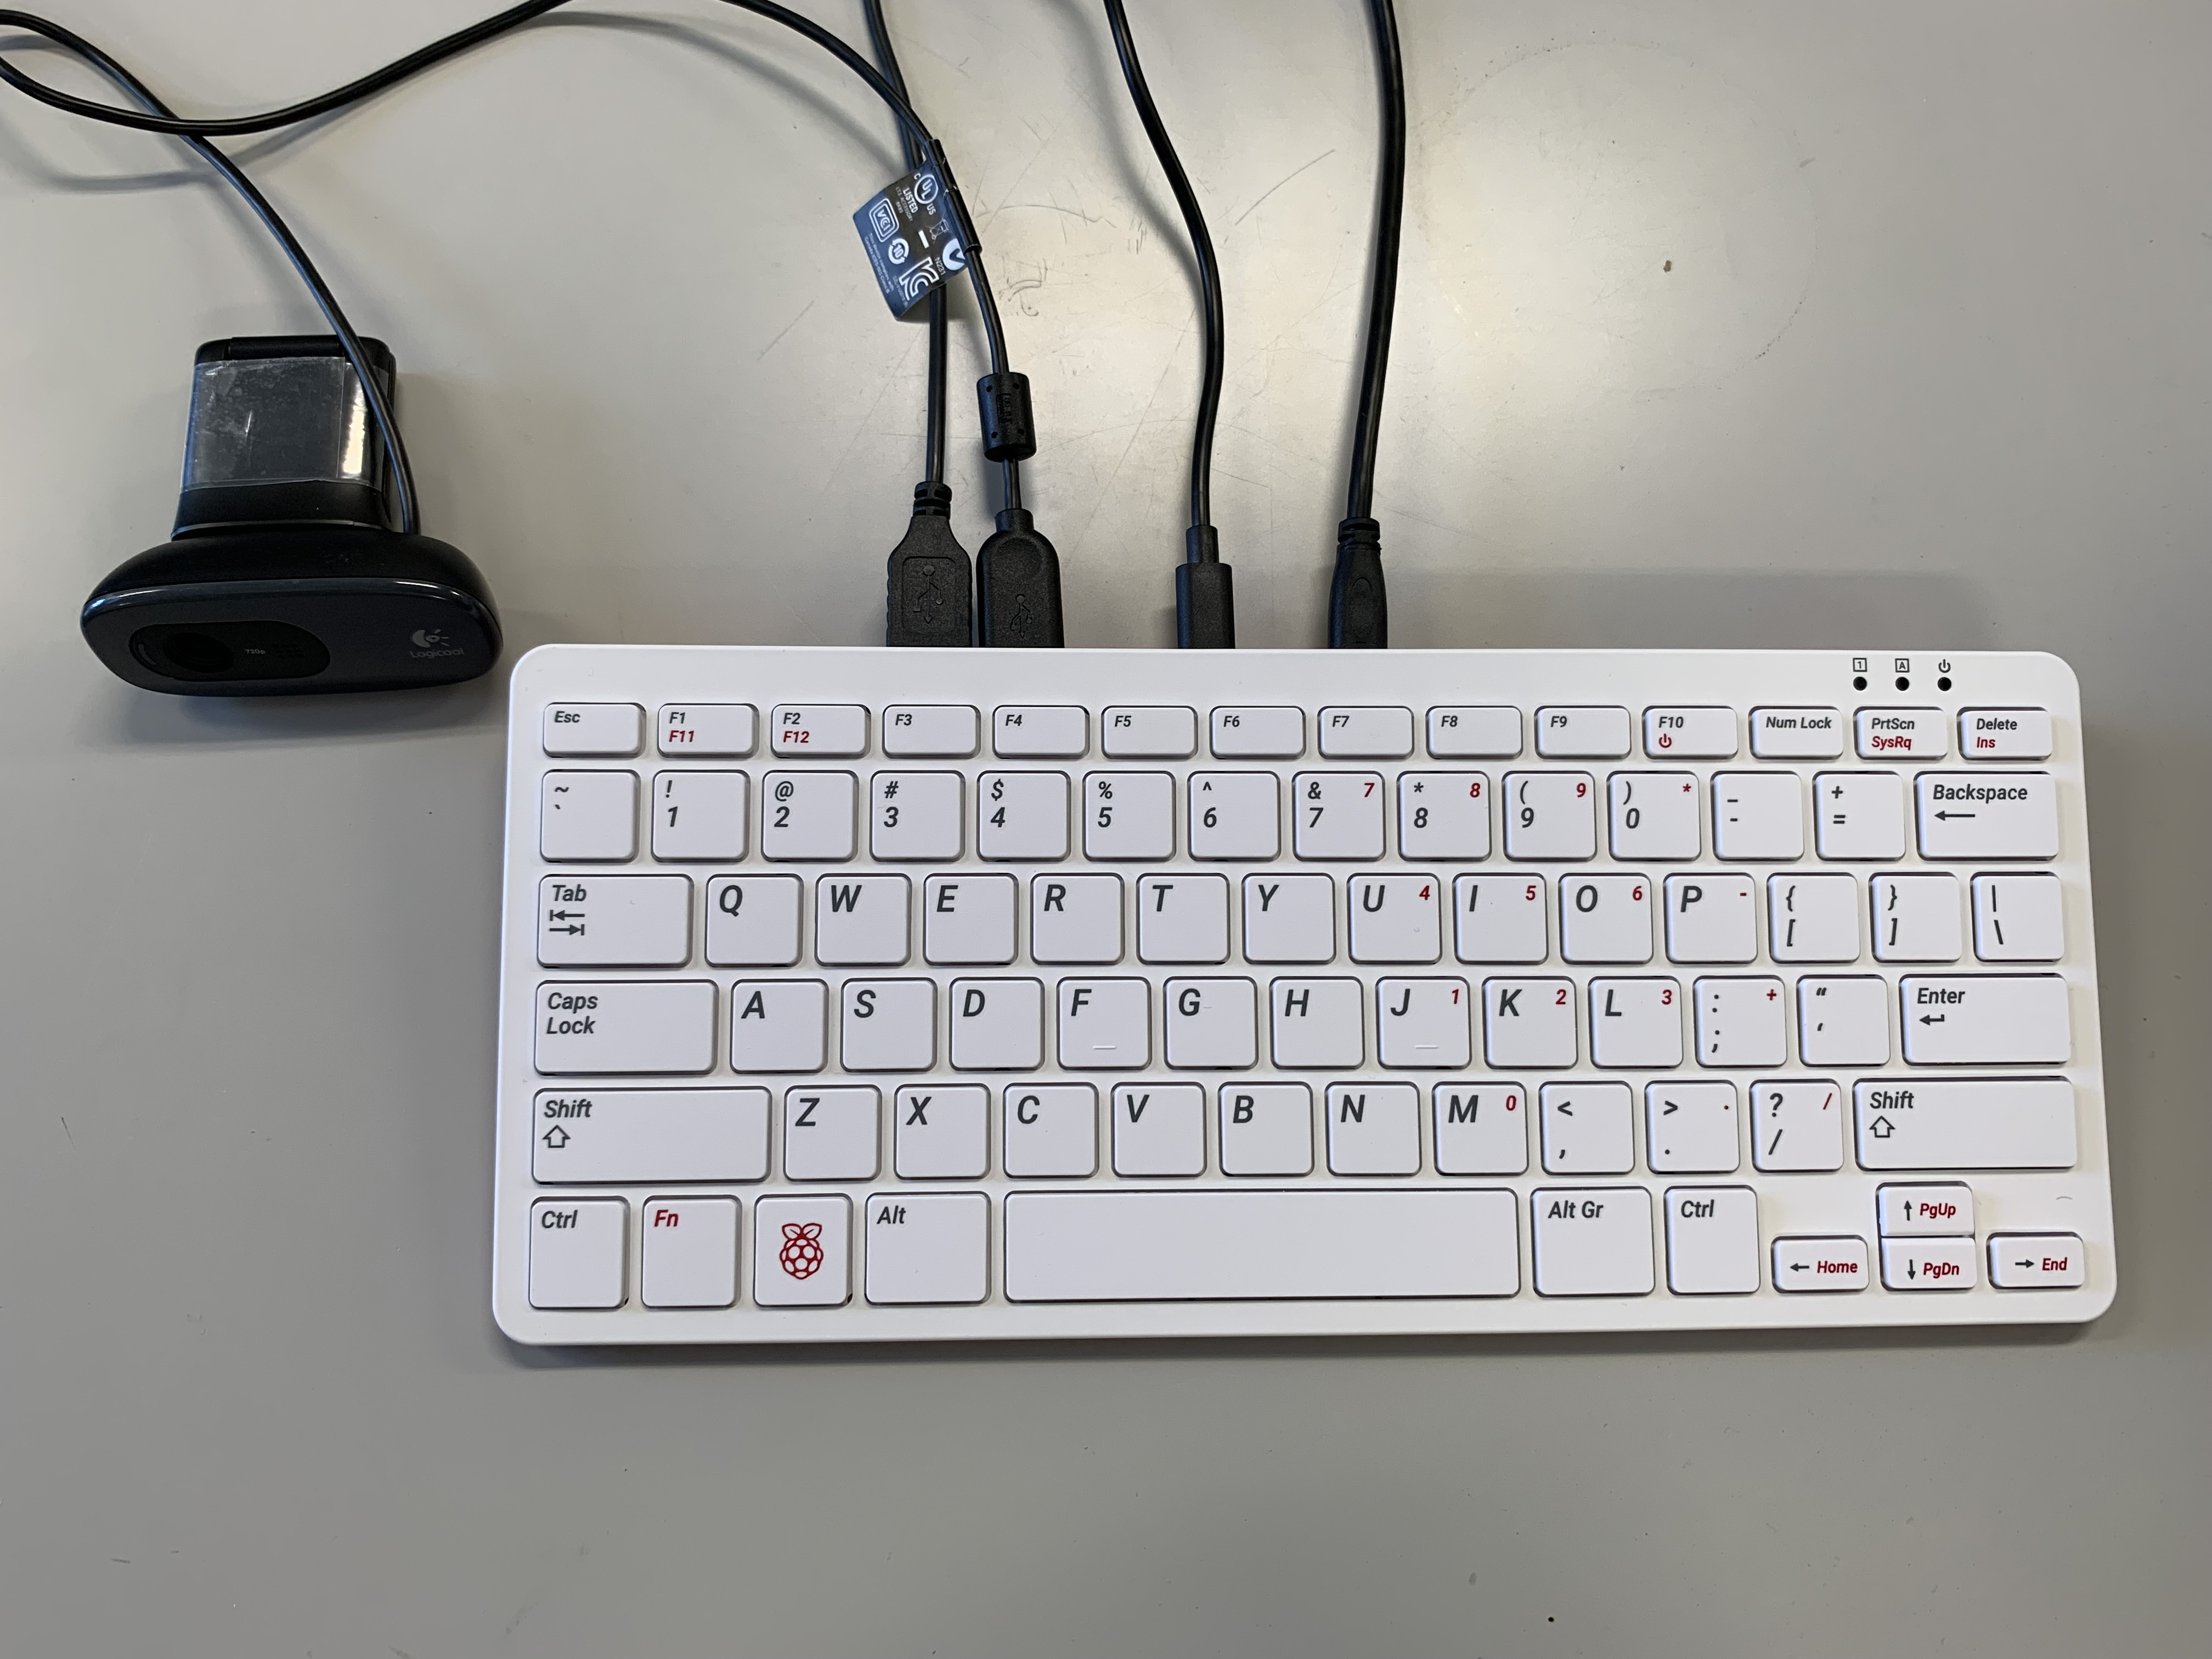
\includegraphics[width=7.904cm]{text01-img/textbook-img112-2023.jpg}
      \caption{Webカメラの\ruby{接続}{せつぞく}}
    }
  \end{minipage}
\end{figure}
\noindent
ウェブカメラを\ruby{接続}{せつぞく}したら、ラズベリーパイからウェブカメラの\ruby{画像}{がぞう}を取得してみましょう。左上のラズベリーのアイコンをクリックします。そこから、サウンドとメディアを\ruby{選択}{せんたく}しVLCメディアプレーヤーをクリックします。

\begin{figure}[hb]
  \centering
  \begin{minipage}{10.917cm}
    {\upshape
      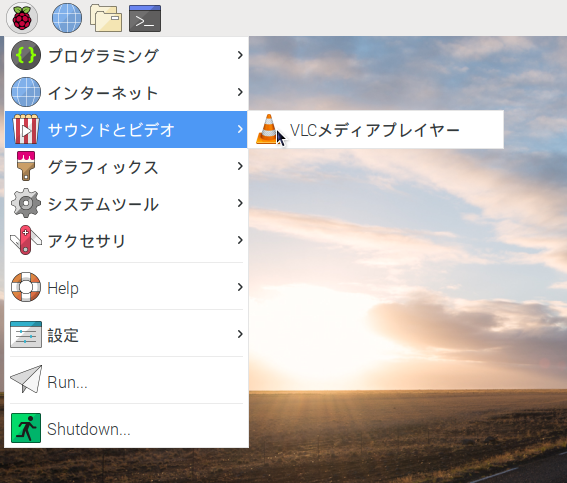
\includegraphics[height=8.715cm]{text01-img/textbook-img113.png}
      \caption{メニューからVLC起動}
    }
  \end{minipage}
\end{figure}
\clearpage

\begin{figure}[ht]
  図~\ref{fig:25}のようにVLCメディアプレーヤーが起動します。

  \centering
  \begin{minipage}{10cm}
    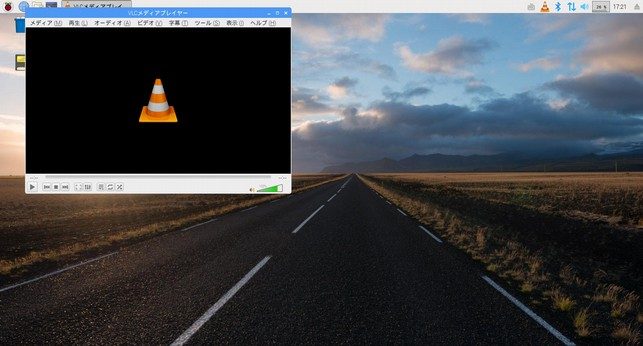
\includegraphics[width=10cm]{text01-img/textbook-img114.jpg}
    \caption{VLC起動画面}\label{fig:25}
  \end{minipage}
  % \flushleft
  % VLCが起動したら\ruby{確認}{かくにん}メッセージが出てきます。

  %後で修正 チェックボックスが出ない \usepackage{amssymb}まで入れたけどダメ
  % \textbf{\textcolor[rgb]{1.0,0.2,0.2}{赤わくで囲われているチェックボックスにチェックマーク(\checked)}}がついていないことを\ruby{確認}{かくにん}して続けるをクリックしてください。

  % \centering
  % \begin{minipage}{7.186cm}
  %   {\upshape
  %     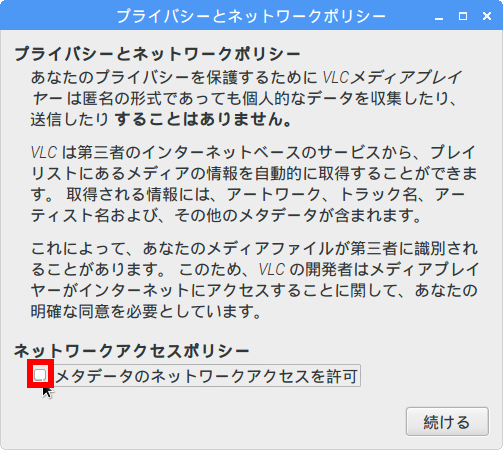
\includegraphics[width=7.2cm]{text01-img/textbook-img115.png}
  %     \caption{\ruby{確認}{かくにん}メッセージ}
  %   }
  % \end{minipage}

  \flushleft
  カメラを開きます。図~\ref{fig:27}のように\textbf{メディア}をクリックして\textbf{キャプチャーデバイスを開く}をクリックします。


  \centering
  \begin{minipage}{8.096cm}
    {\upshape
      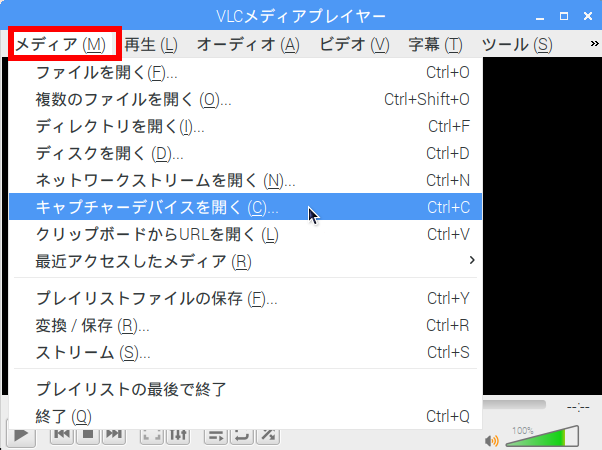
\includegraphics[width=8.0cm]{text01-img/textbook-img116.png}
      \caption{キャプチャデバイスをひらく}\label{fig:27}
    }
  \end{minipage}

  \flushleft
  図~\ref{fig:28}のような画面がでてきます。
  赤線で囲われている\textbf{キャプチャーモード}を
  \textbf{Video camera}にして
  青線で囲われている\textbf{\ruby{再生}{さいせい}}をクリックします。

  \centering
  \begin{minipage}{10cm}
    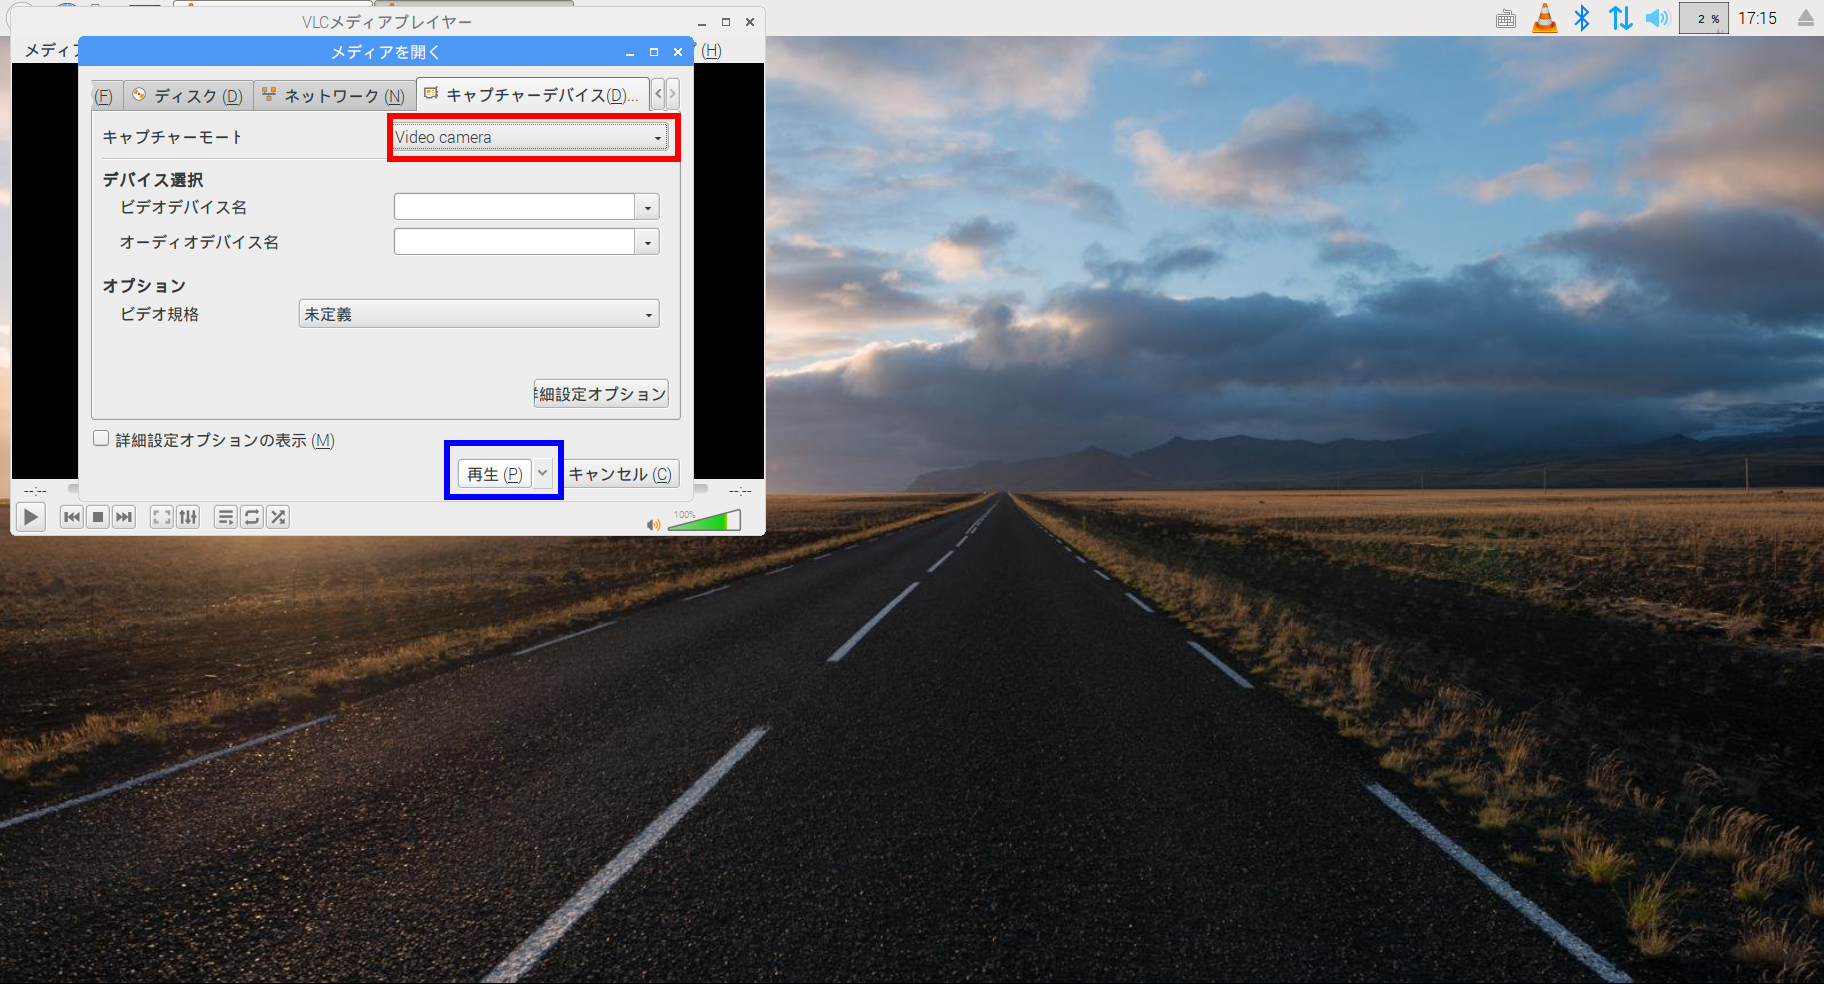
\includegraphics[width=10cm]{text01-img/textbook-img117.png}
    \caption{キャプチャーデバイスを開く画面}\label{fig:28}
  \end{minipage}


\end{figure}
% \clearpage


\begin{figure}[ht]
  % 図~\ref{fig:28}のような画面がでてきます。
  % 赤線で囲われている\textbf{キャプチャーモード}を
  % \textbf{Video camera}にして
  % 青線で囲われている\textbf{\ruby{再生}{さいせい}}をクリックします。


  % \centering
  % \begin{minipage}{10cm}
  %   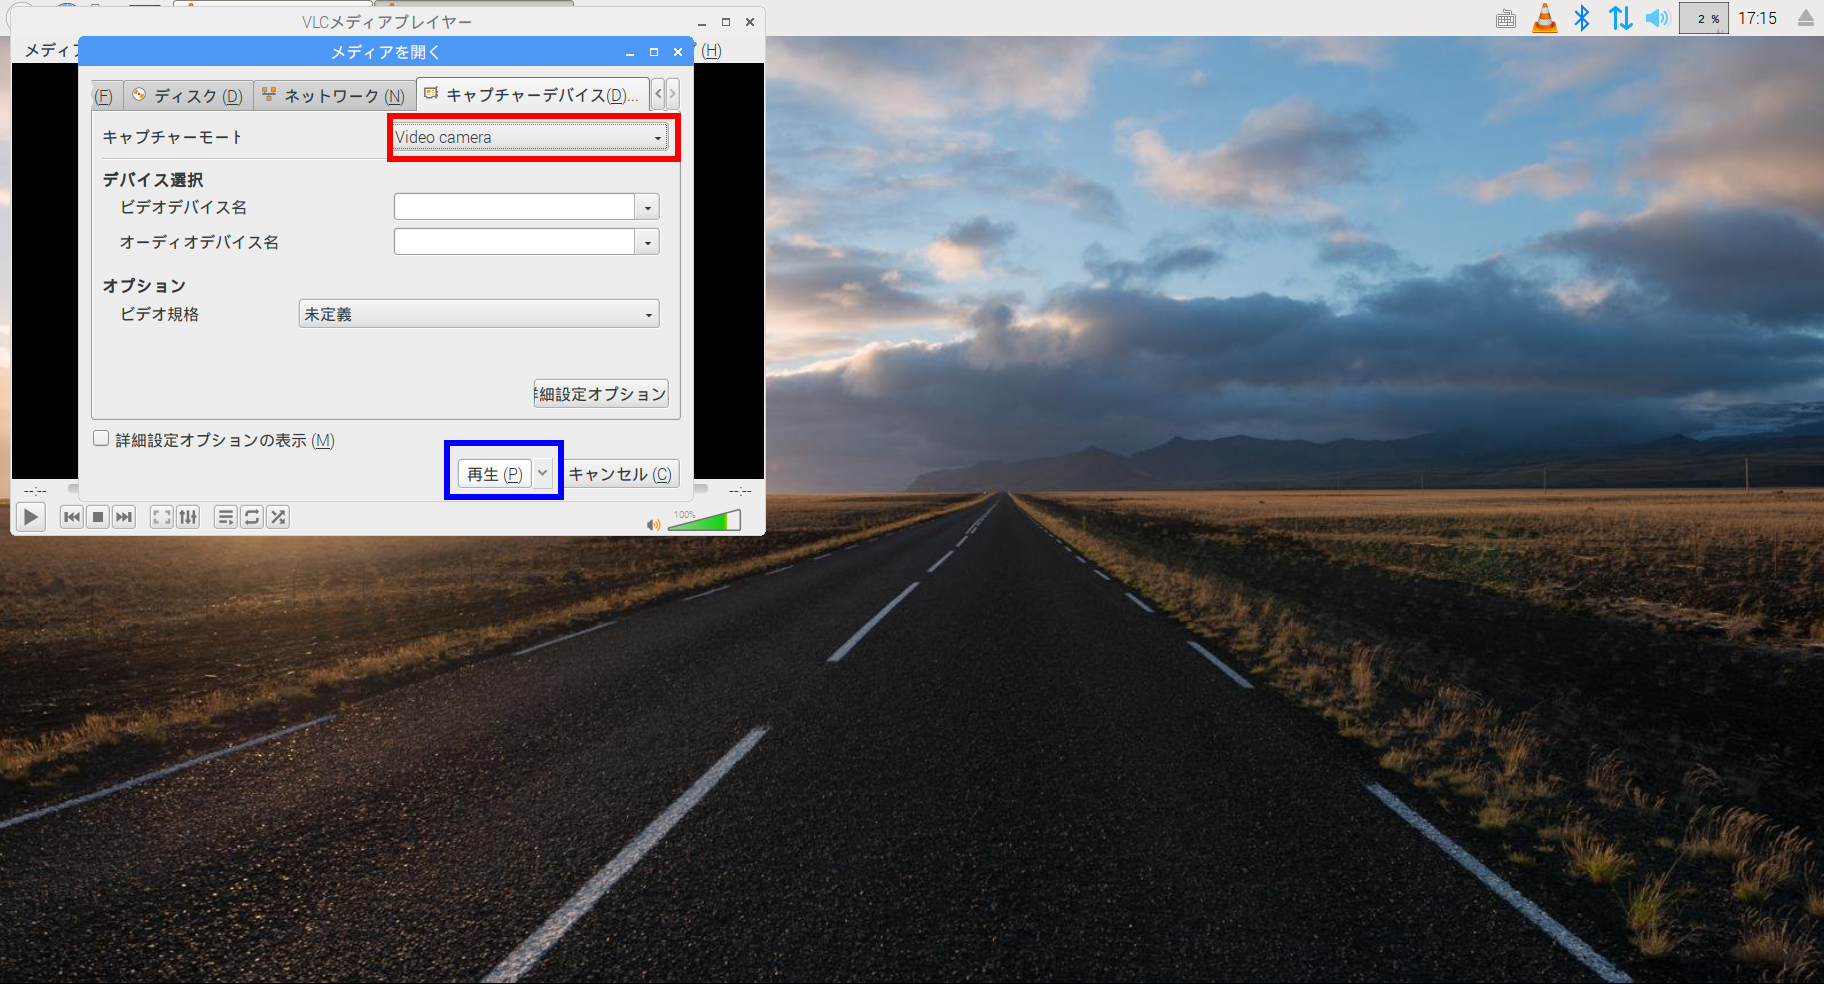
\includegraphics[width=10cm]{text01-img/textbook-img117.png}
  %   \caption{キャプチャーデバイスを開く画面}\label{fig:28}
  % \end{minipage}

  \flushleft
  しばらくすると、カメラの\ruby{画像}{がぞう}が見えるようになります。

  \centering
  \begin{minipage}{10cm}
    {\upshape
      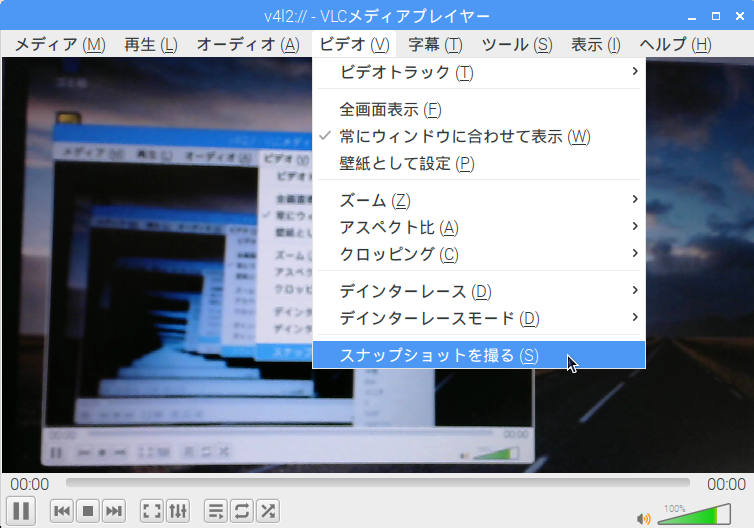
\includegraphics[width=10cm]{text01-img/textbook-img118.png}
      \caption{スナップショット\ruby{撮影}{さつえい}}
    }
  \end{minipage}

  \flushleft
  次に、カメラでさつえいしてみましょう。ビデオをクリックしてスナップショットを撮るをクリックします。


  \centering
  \begin{minipage}{10cm}
    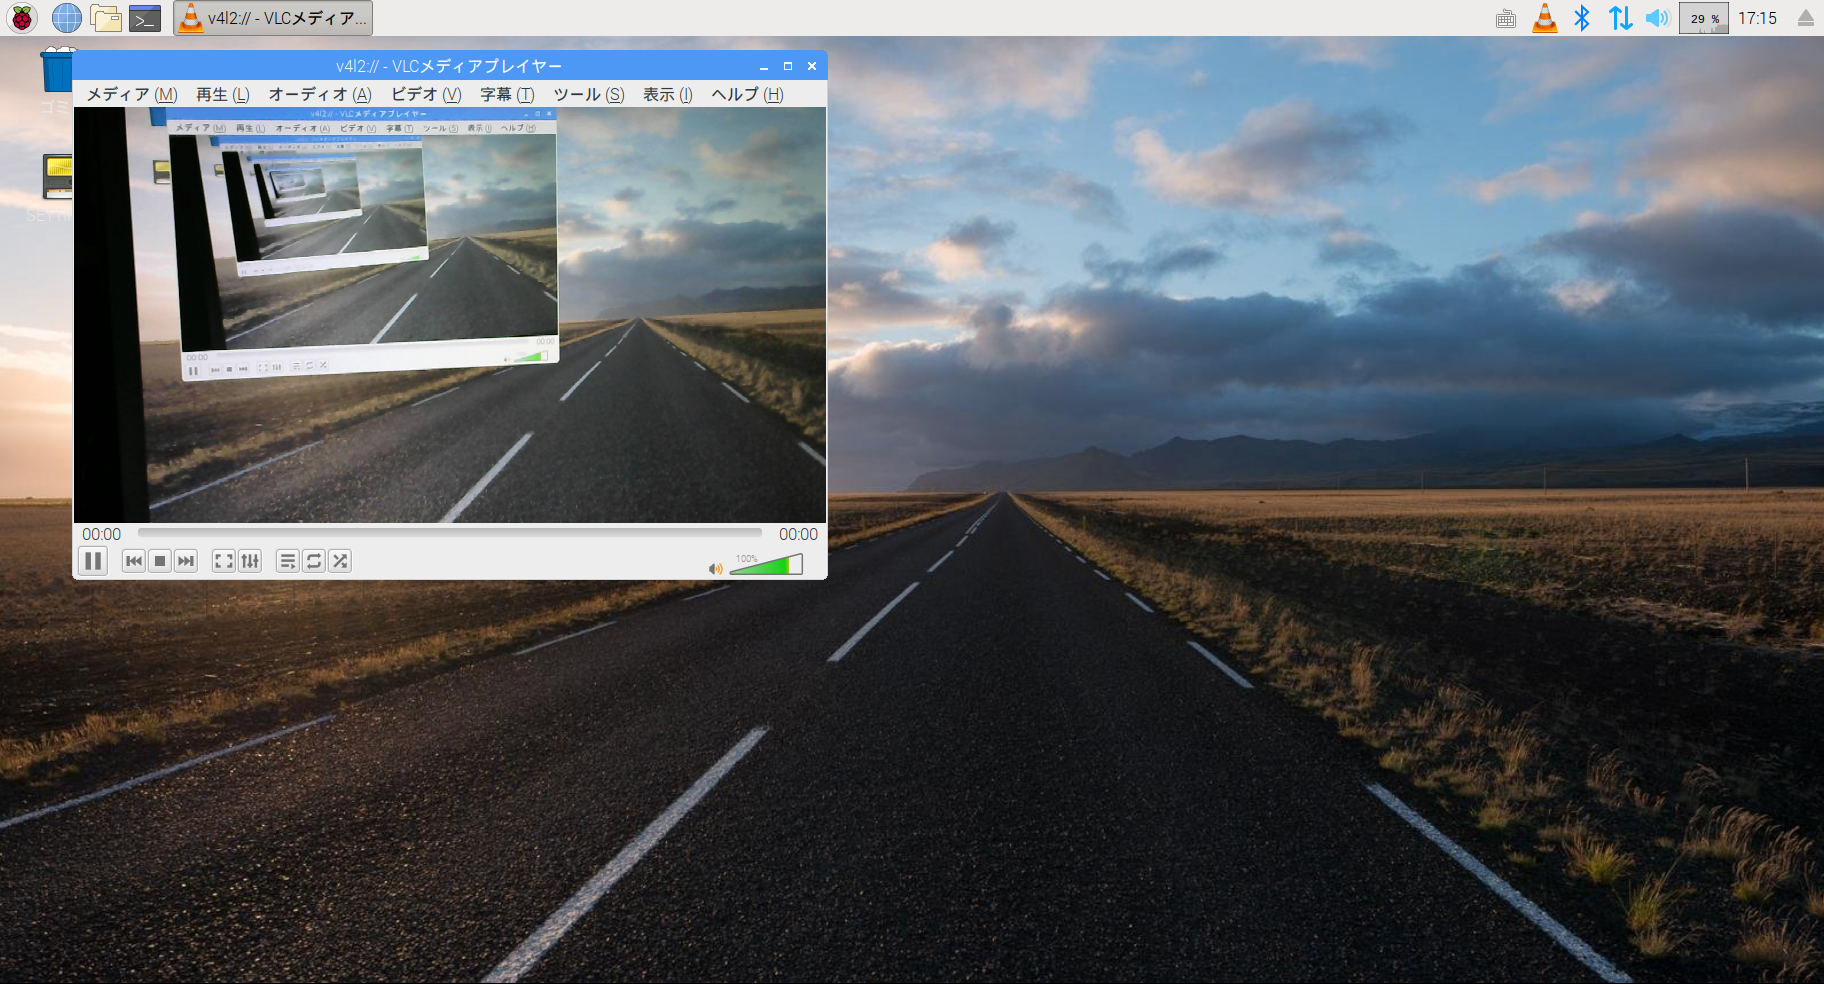
\includegraphics[width=10cm]{text01-img/textbook-img119.png}
    {\upshape
      \caption{カメラ入力}
    }
  \end{minipage}

  \flushleft
  黒線の四角に囲われたように\ruby{保存}{ほぞん}場所が表示され、そこへ\ruby{画像}{がぞう}が\ruby{保存}{ほぞん}されます。

  \centering
  \begin{minipage}{10cm}
    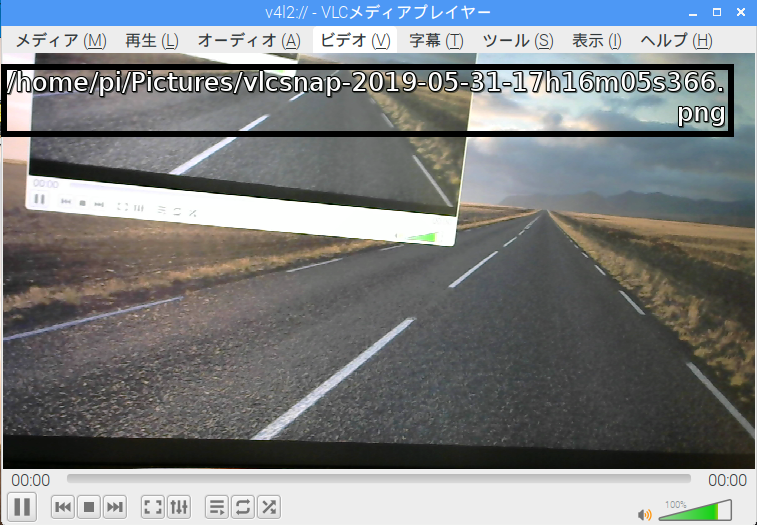
\includegraphics[width=10cm]{text01-img/textbook-img120.png}
    \caption{スナップショット\ruby{保存}{ほぞん}}
  \end{minipage}

\end{figure}
\clearpage

\vspace*{-1.8cm}
\begin{figure}
  % 黒線の四角に囲われたように\ruby{保存}{ほぞん}場所が表示され、そこへ\ruby{画像}{がぞう}が\ruby{保存}{ほぞん}されます。

  % \centering
  % \begin{minipage}{10cm}
  %   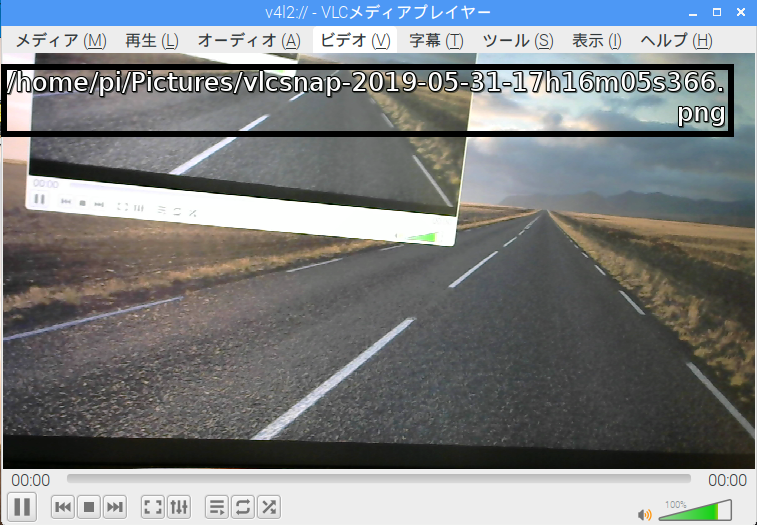
\includegraphics[width=10cm]{text01-img/textbook-img120.png}
  %   \caption{スナップショット\ruby{保存}{ほぞん}}
  % \end{minipage}
  % \bigskip

  \flushleft
  初期\ruby{状態}{じょうたい}ではPicturesの下に\ruby{保存}{ほぞん}されます。\ruby{確認}{かくにん}してみましょう。

  \centering
  \begin{minipage}{10cm}
    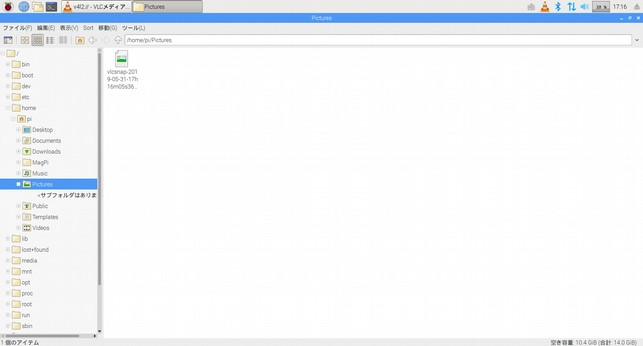
\includegraphics[width=10cm]{text01-img/textbook-img121.jpg}
    \caption{\ruby{画像}{がぞう}\ruby{撮影}{さつえい}場所}
  \end{minipage}


  \bigskip

  \flushleft
  とった\ruby{画像}{がぞう}を\ruby{確認}{かくにん}してみましょう。図~\ref{fig:33}の赤わくで囲ってあるものがとった写真です。ダブルクリックをすると、\ruby{画像}{がぞう}を開いて見ることができます。



  \centering
  \begin{minipage}{10cm}
    {\upshape
      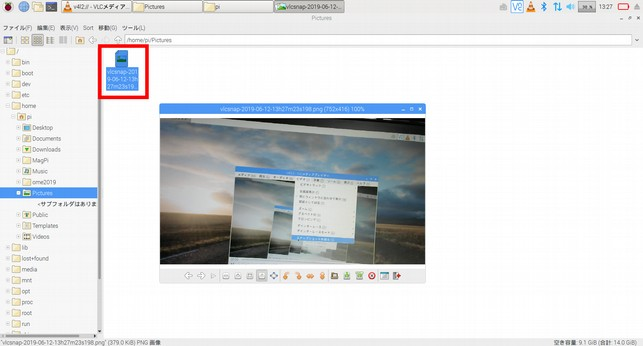
\includegraphics[width=10cm]{text01-img/textbook-img122.jpg}
      \caption{とった\ruby{画像}{がぞう}を開く}\label{fig:33}
    }
  \end{minipage}
\end{figure}

\bigskip

\clearpage


\begin{figure}[ht]
  \subsection{例題 1-17 \ruby{画像}{がぞう}に絵をかこう}

  “GIMP”ソフトを立ち上げて、色付きの筆で自分の顔写真に絵をかこう

  \ruby{画像}{がぞう}を開いて、色を\ruby{選択}{せんたく}、お絵かきツールの筆を選んで書くよ

  \textbf{考え方}

  \begin{minipage}{0.4\textwidth}
    \centering
    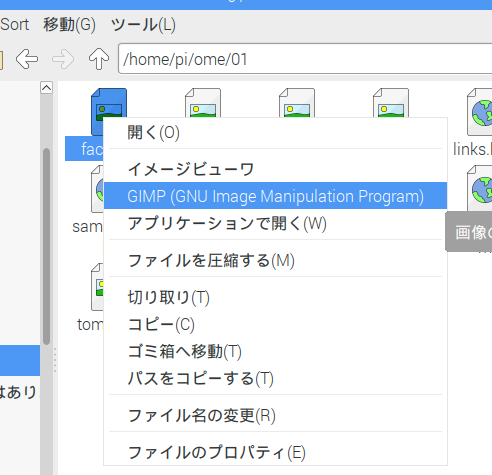
\includegraphics[width=\linewidth]{text01-img/textbook-img124.png}\\
    \flushleft
    1 \ruby{編集}{へんしゅう}したい\ruby{画像}{がぞう}ファイルを右クリックして

    【次で開く】→【GIMP】をクリック
  \end{minipage}
  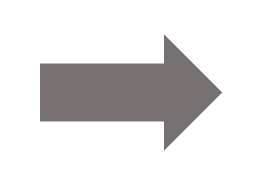
\includegraphics[width=2cm]{text01-img/textbook-img128.png}
  \begin{minipage}{0.4\textwidth}
    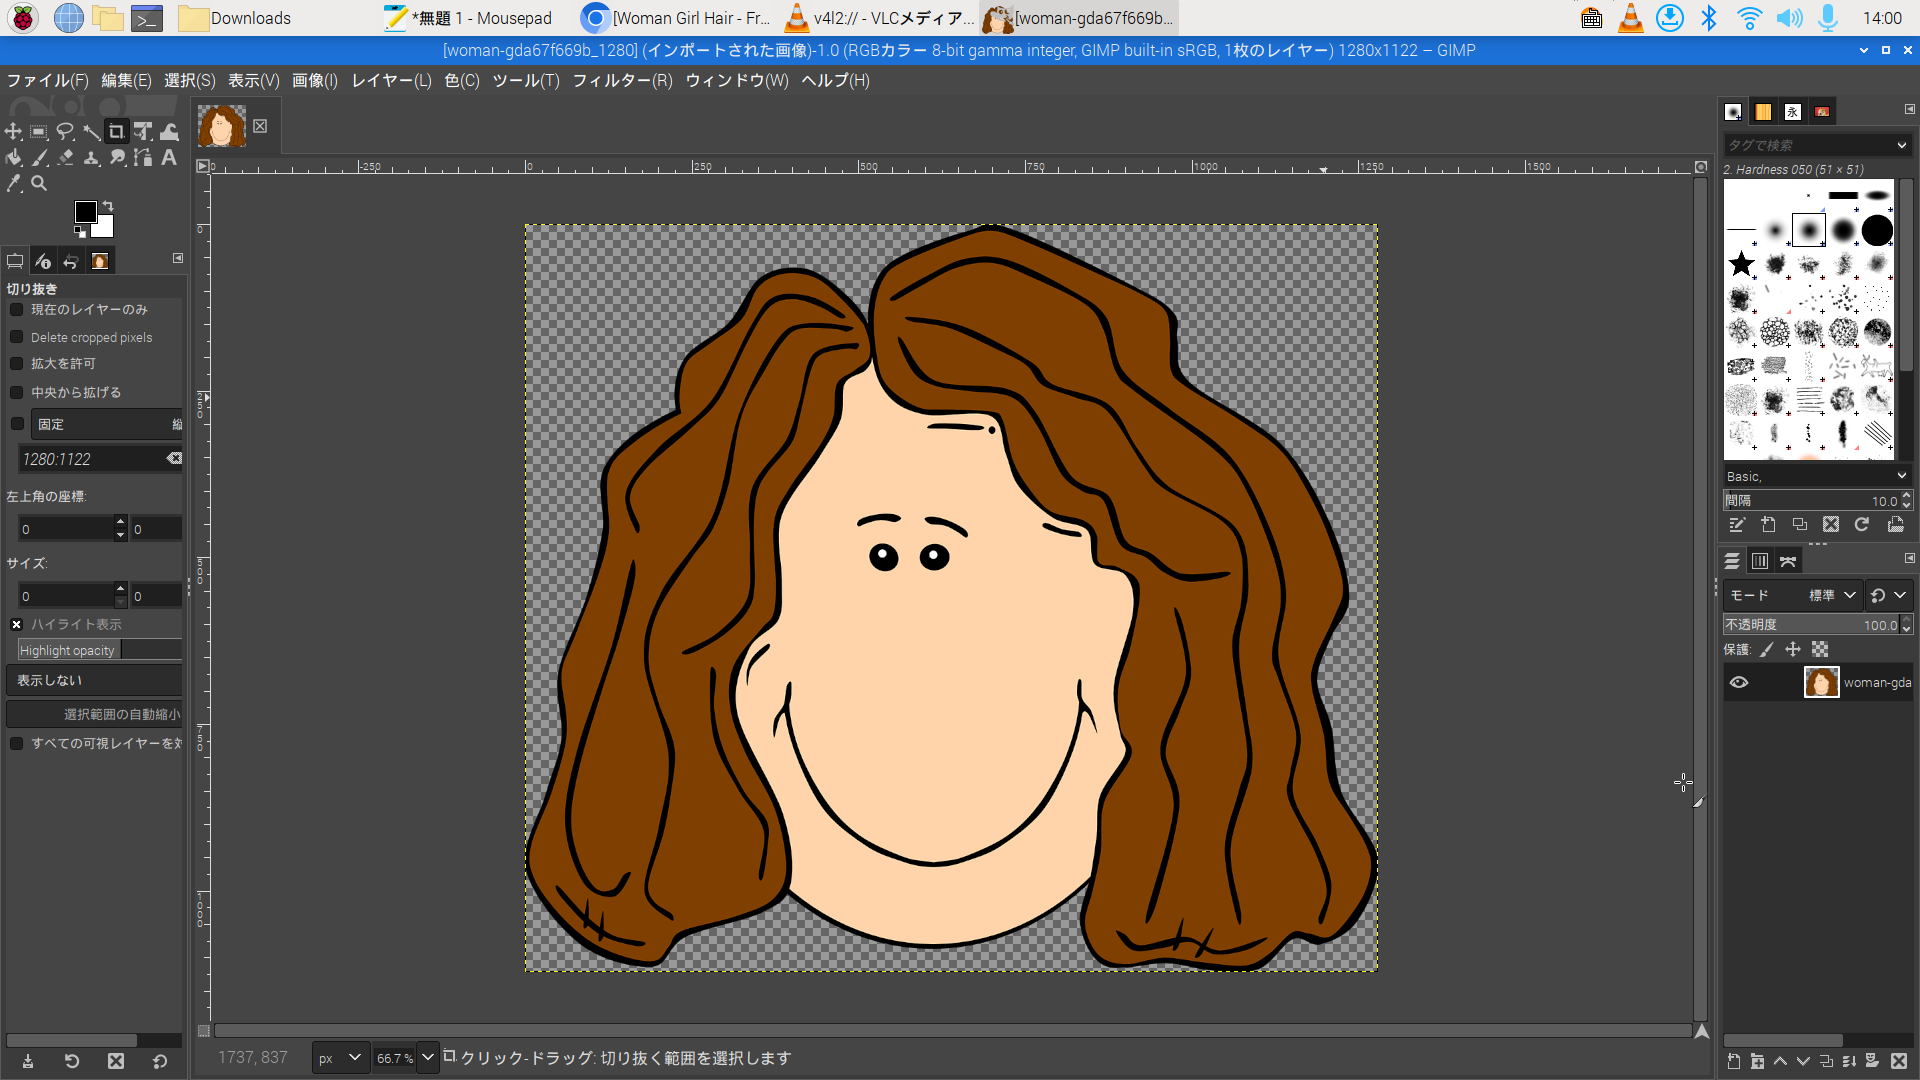
\includegraphics[width=\linewidth]{text01-img/textbook-img125.png}\\
      2 \ruby{画像}{がぞう}\ruby{編集}{へんしゅう}モードになるよ
  \end{minipage}
  
  \begin{minipage}{0.4\textwidth}
    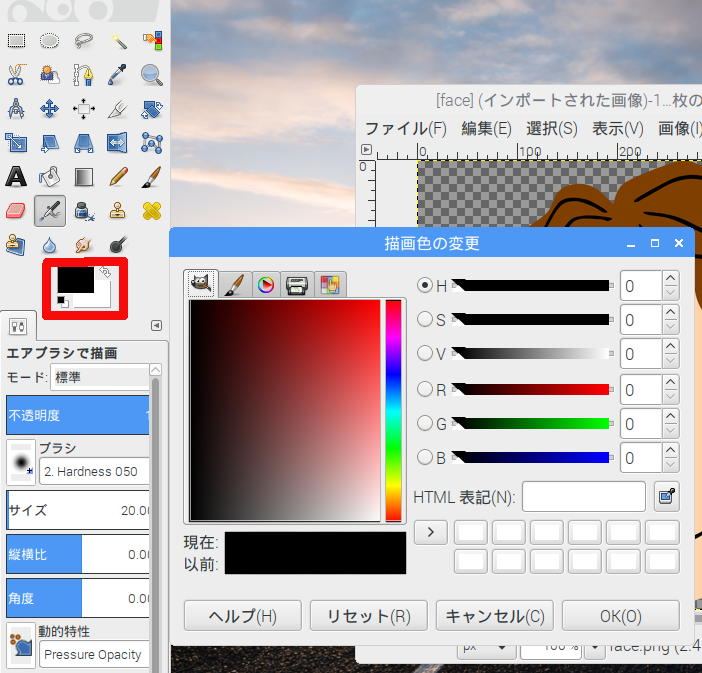
\includegraphics[width=\linewidth]{text01-img/textbook-img129.png}\\
    3 画面左上の、赤い丸で囲まれている部分をクリック
  \end{minipage}
  \hspace{2cm}
  \begin{minipage}{0.4\textwidth}
    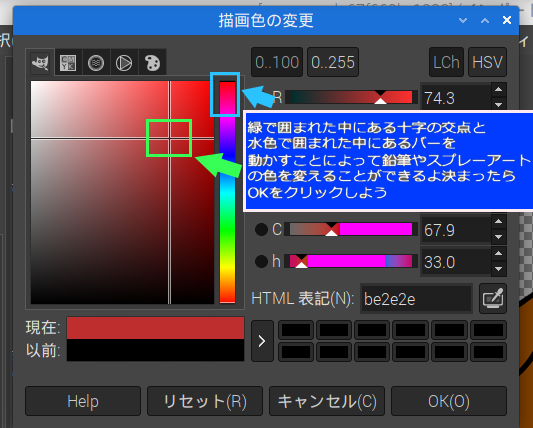
\includegraphics[width=\linewidth]{text01-img/textbook-img126.png}\\
    4 色を変更しよう

    好きな色を選んでOKを\ruby{押}{お}します\\
  \end{minipage}

  \begin{minipage}{0.4\textwidth}
    5 今回は色を赤にしました。赤い丸で囲んであるところの色が赤に変わっていることを\ruby{確認}{かくにん}してください。
  \end{minipage}
  \hspace{2cm}
  \begin{minipage}{0.4\textwidth}
    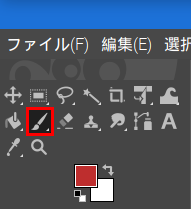
\includegraphics[width=\linewidth]{text01-img/textbook-img127.png}
    6 次にお絵かきツールを選びます。

    赤色で囲われているところをクリックしてください。これで色付きの筆が使えるようになります。

  \end{minipage}
\end{figure}
\clearpage


\begin{figure}[ht]
  \textbf{考え方(続き)}

  \begin{minipage}{0.4\textwidth}
    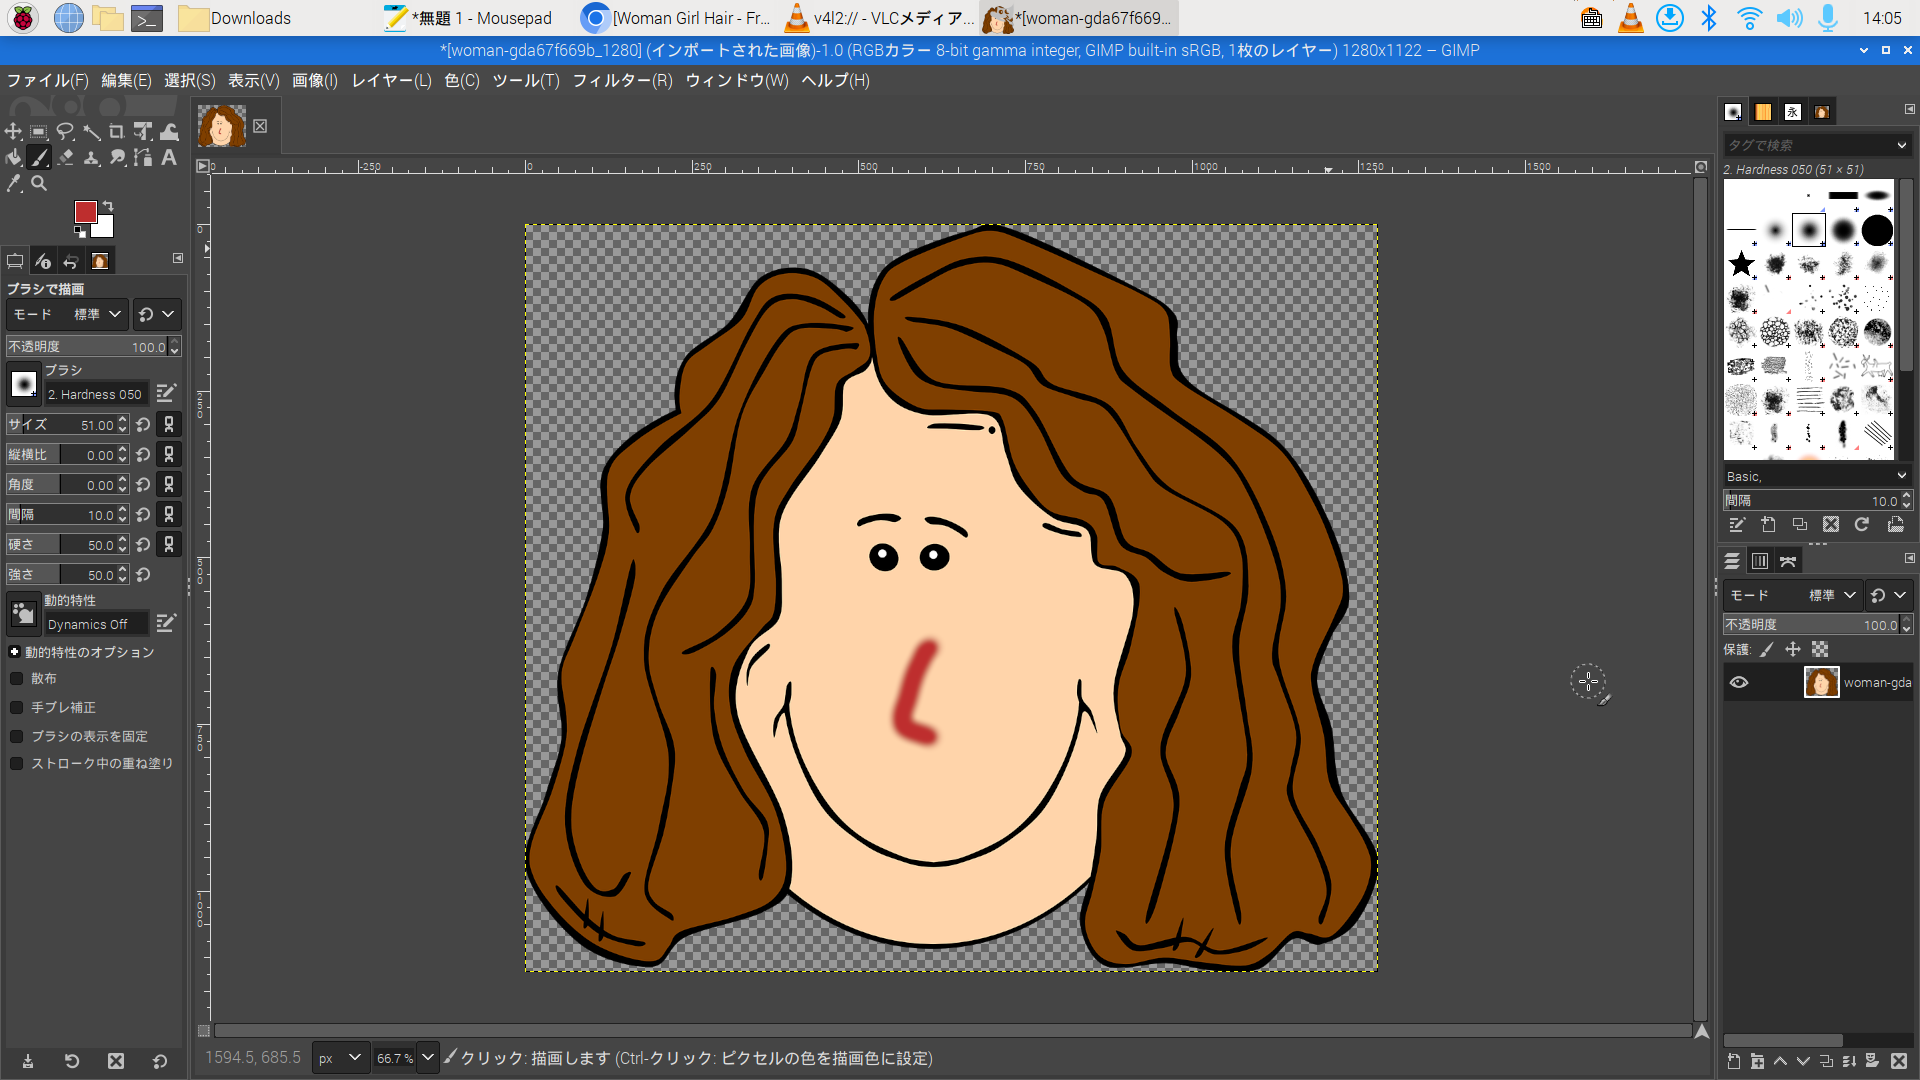
\includegraphics[width=\linewidth]{text01-img/textbook-img131.png}\\
    8 左クリックをおしながら\ruby{画像}{がぞう}の上を\ruby{移動}{いどう}させると筆でお絵かきができます。いたずら書きをしてみてください
    % 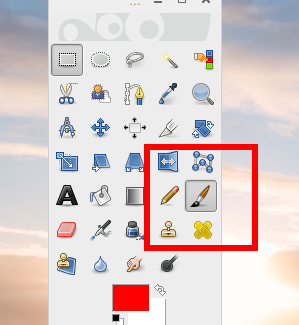
\includegraphics[width=\linewidth]{text01-img/textbook-img130.png}\\
    %   7 ツール\ruby{一覧}{いちらん}の下の文字が「ブラシで\ruby{描画}{びょうが}」に変わったことを\ruby{確認}{かくにん}しましょう。これで筆が使えるようになりました。
  \end{minipage}
  \hspace{1cm}
  \begin{minipage}{0.6\textwidth}
    % 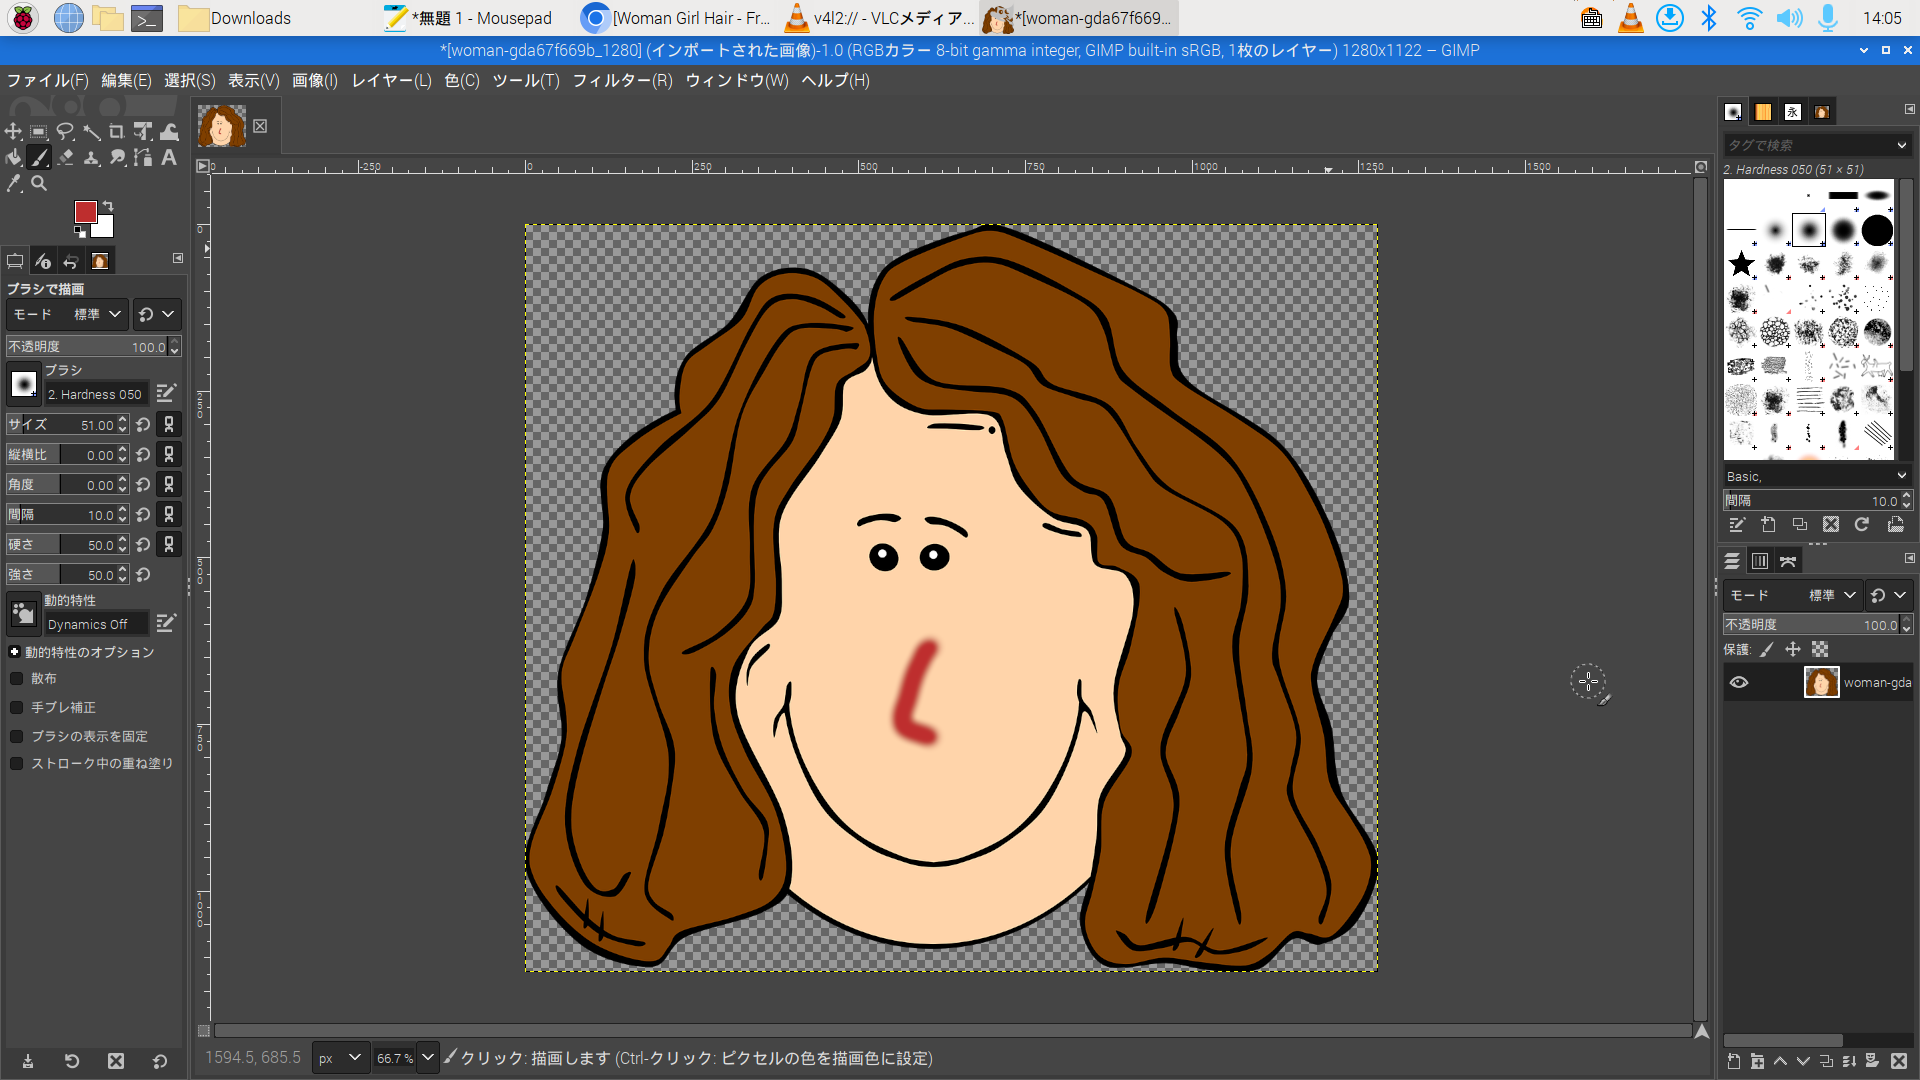
\includegraphics[width=\linewidth]{text01-img/textbook-img131.png}\\
    % 8 左クリックをおしながら\ruby{画像}{がぞう}の上を\ruby{移動}{いどう}させると筆でお絵かきができます。いたずら書きをしてみてください
  \end{minipage}

  \bigskip

  \begin{minipage}{\textwidth}
    \begin{minipage}{6.984cm}
      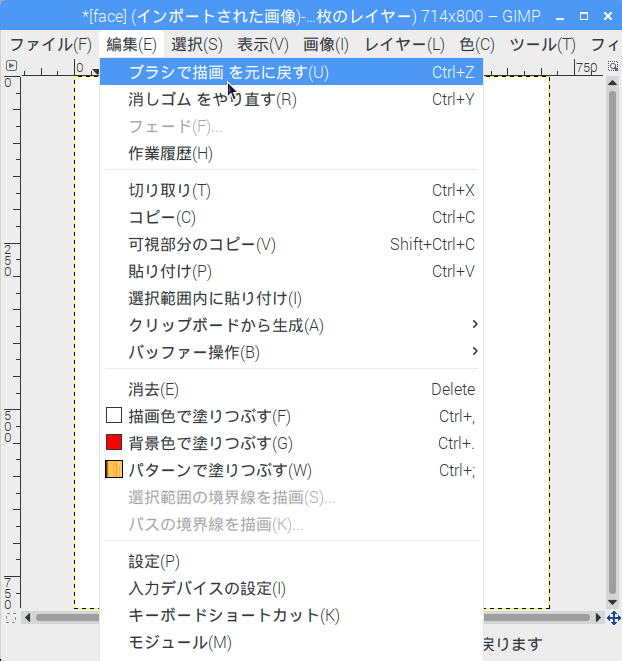
\includegraphics[width=6.228cm]{text01-img/textbook-img132.png}\\
      9 \ruby{間違}{まちが}えてしまって、もとに\ruby{戻}{もど}したいとなったらメニューの\ruby{編集}{へんしゅう}からもとに\ruby{戻}{もど}すをクリックします。
    \end{minipage}
    \hfill
    \begin{minipage}{8.966cm}
      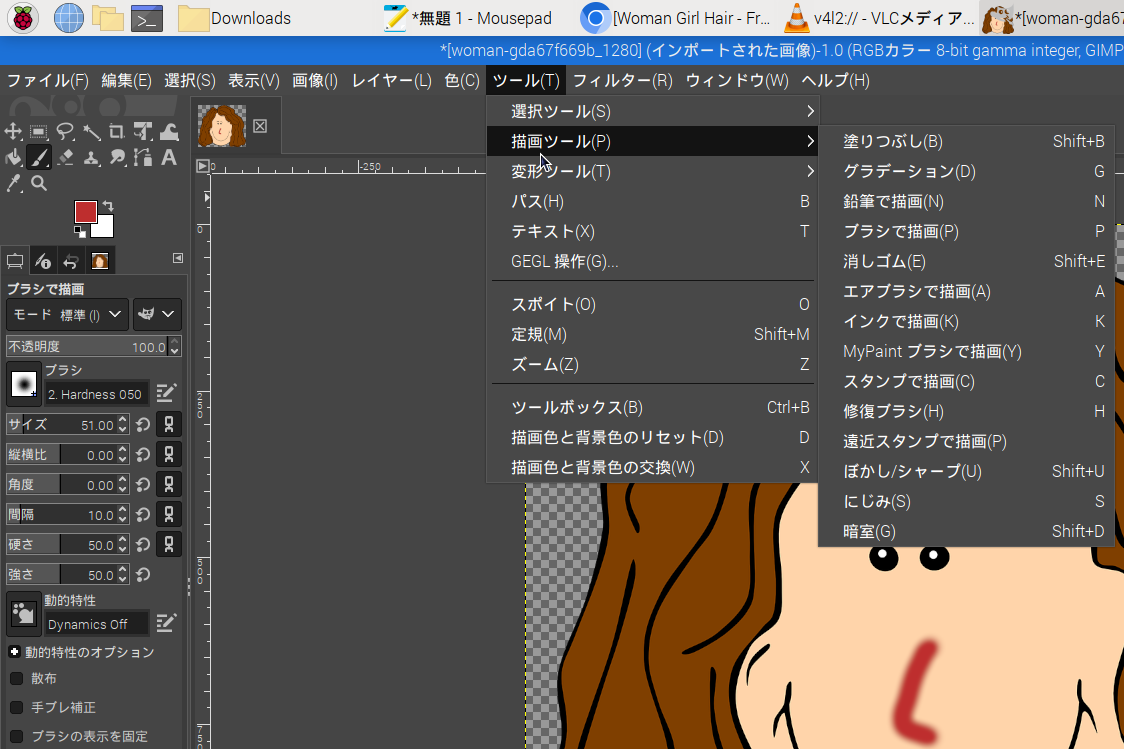
\includegraphics[width=8.881cm,height=4.997cm]{text01-img/textbook-img133.png}\\
      10 赤い\ruby{枠}{わく}で囲まれたブラシのアイコンを右クリックすると、別のお絵描きツールを選ぶことができるよ。\ruby{鉛筆}{えんぴつ}、インクを試してみよう。書き方はいっしょで左クリックをを\ruby{押}{お}しながら\ruby{移動}{いどう}だよ
    \end{minipage}
  \end{minipage}
\end{figure}
\clearpage


\begin{figure}
  \textbf{考え方(続き)}


  \ruby{編集}{へんしゅう}しおわったら書き出しをします。

  \centering
  \begin{minipage}{\textwidth}
    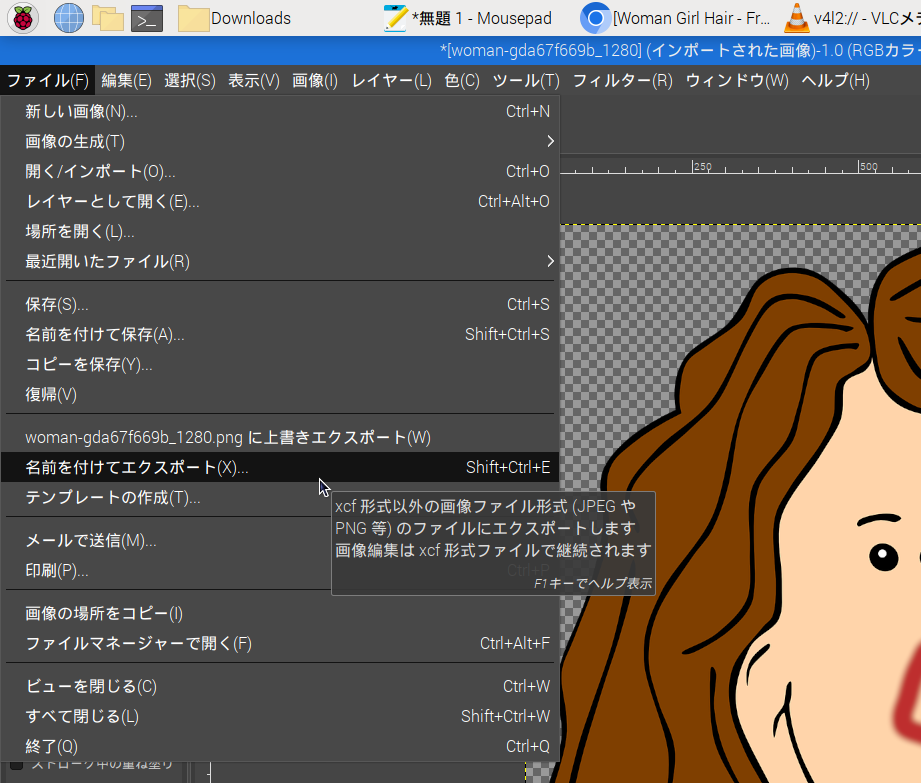
\includegraphics[width=0.5\textwidth]{text01-img/textbook-img138.png}\\
    11 \ruby{編集}{へんしゅう}がおわったら

    ファイルから名前を付けてエクスポートをクリック
  \end{minipage}

  \bigskip


  \begin{minipage}{\textwidth}
    \begin{minipage}{0.45\textwidth}
      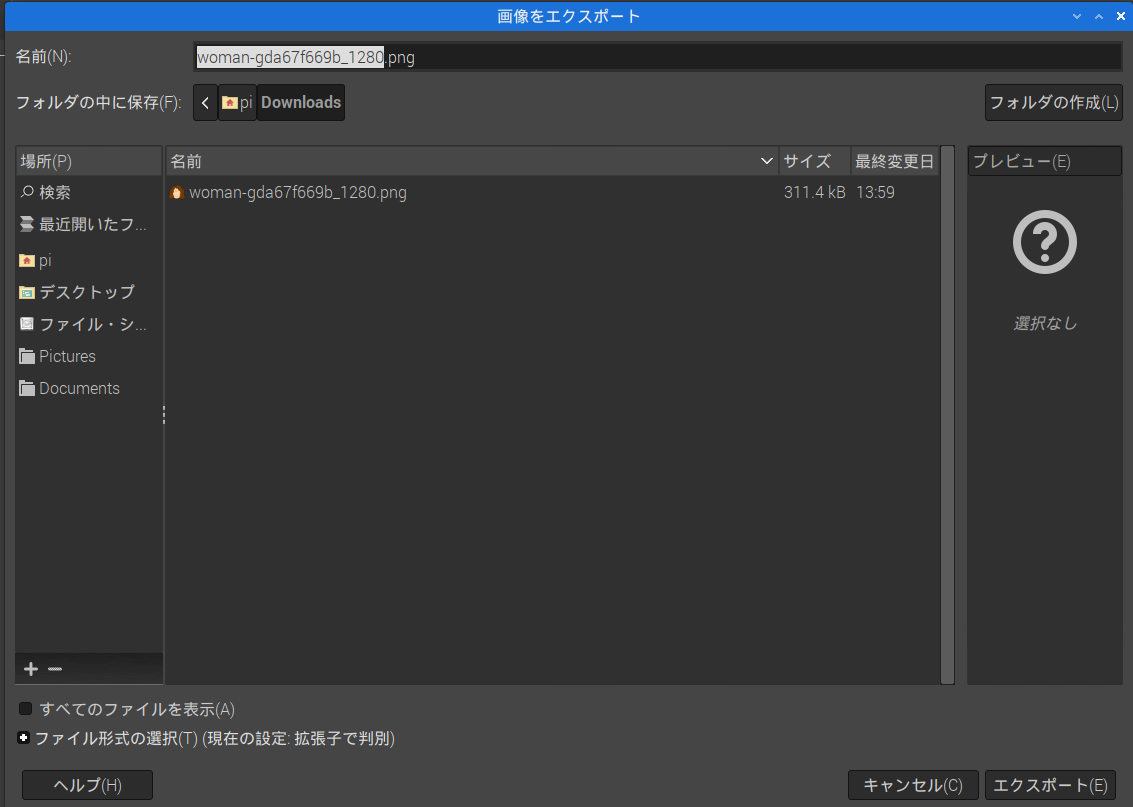
\includegraphics[width=\linewidth]{text01-img/textbook-img137.png}\\
      12 下のエクスポートをクリック(.jpegファイルから\ruby{編集}{へんしゅう}したならば12へ)
    \end{minipage}
    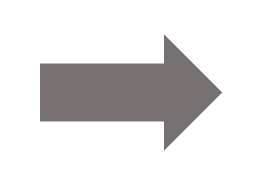
\includegraphics[width=1.919cm]{text01-img/textbook-img135.png}
    \begin{minipage}{0.45\textwidth}
      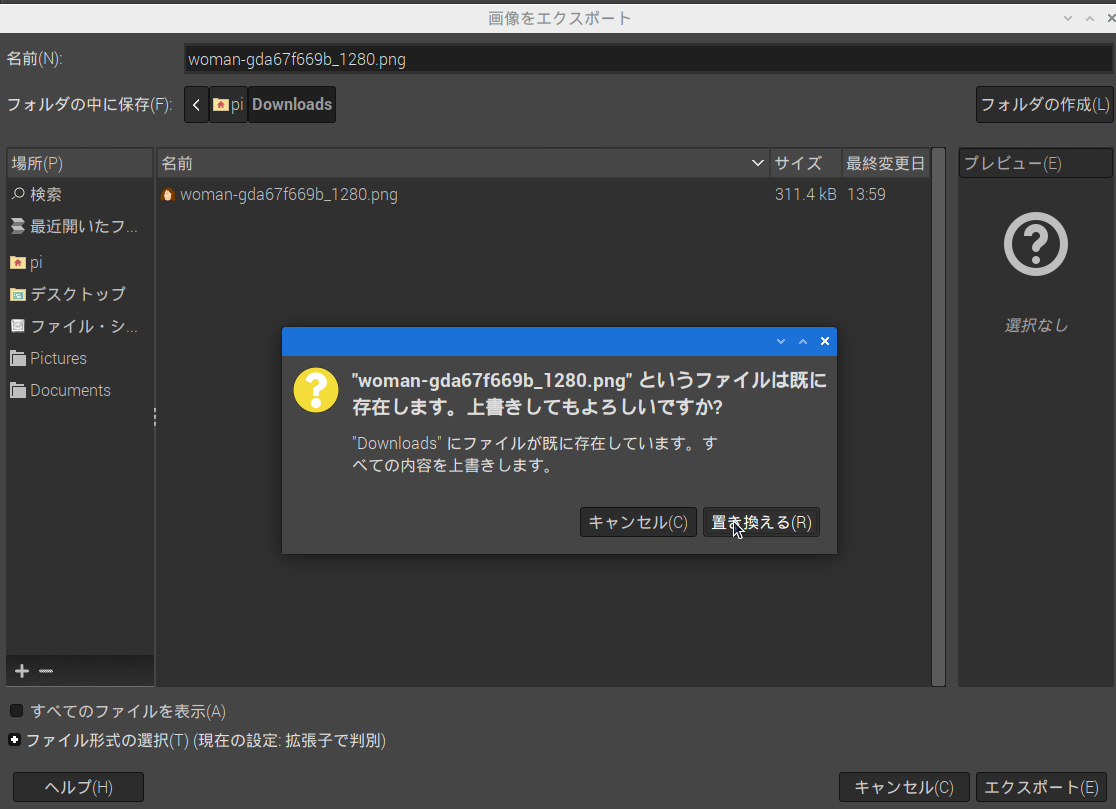
\includegraphics[width=\linewidth]{text01-img/textbook-img136.png}\\
      13 置き換えるをクリック
    \end{minipage}
  \end{minipage}

  \bigskip


  \begin{minipage}{\textwidth}
    \begin{minipage}{0.45\textwidth}
      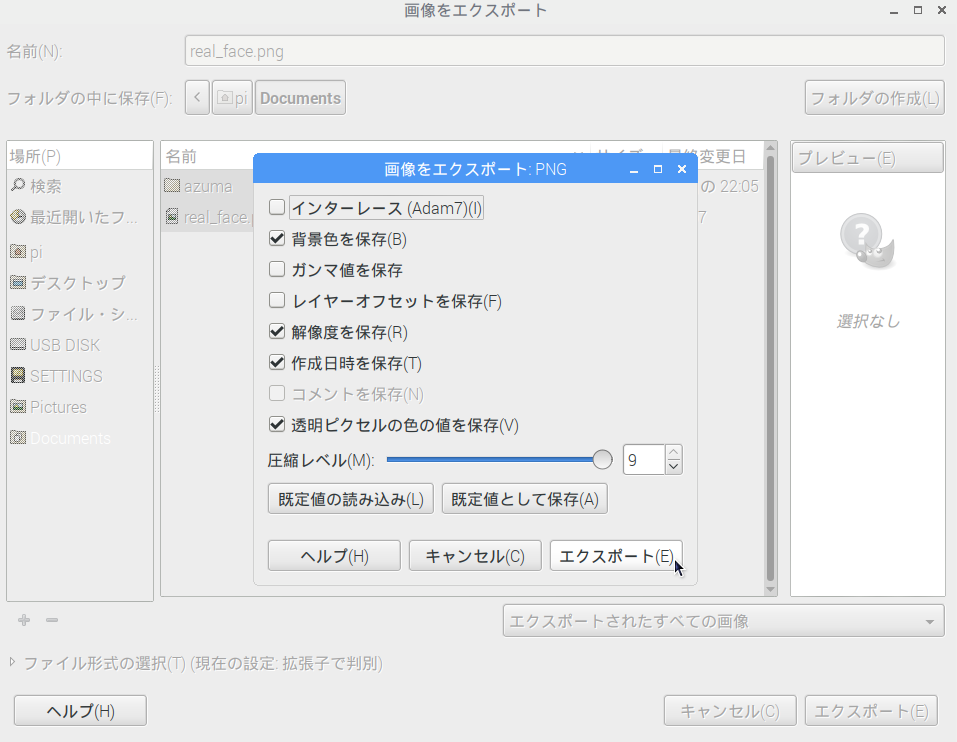
\includegraphics[width=\linewidth]{text01-img/textbook-img134.png}\\
      14 エクスポートをクリック
    \end{minipage}
    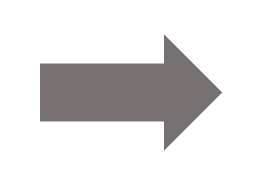
\includegraphics[width=1.919cm]{text01-img/textbook-img135.png}
    \begin{minipage}{0.45\textwidth}
      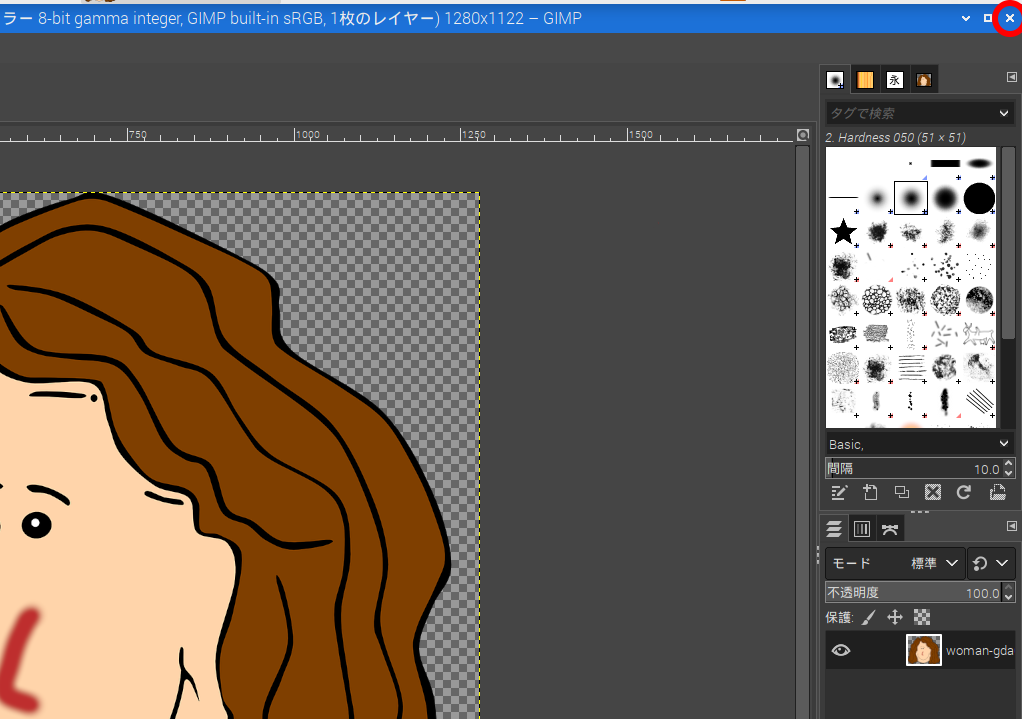
\includegraphics[width=\linewidth]{text01-img/textbook-img1030.png}\\
      15 右上の赤い丸で囲まれた×ボタンをを\ruby{押}{お}して、\ruby{画像}{がぞう}\ruby{編集}{へんしゅう}ツールを\ruby{閉}{と}じよう
    \end{minipage}
  \end{minipage}
\end{figure}
\clearpage


\begin{figure}
  \textbf{考え方(続き)}

  \begin{minipage}{\textwidth}
    \begin{minipage}{0.45\linewidth}
      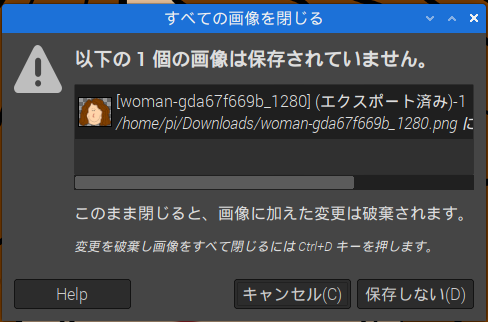
\includegraphics[width=\linewidth]{text01-img/textbook-img1031.png}\\
      16 「\ruby{保存}{ほぞん}されていません」というウィンドウがでます。これは、先ほど「エクスポート」したものとは別のことを言っていて、
      \ruby{画像}{がぞう}自体は\ruby{保存}{ほぞん}されています。なので、気にせず「\ruby{保存}{ほぞん}しない」をクリックしましょう
    \end{minipage}
    \hfill
    \begin{minipage}{0.45\linewidth}
      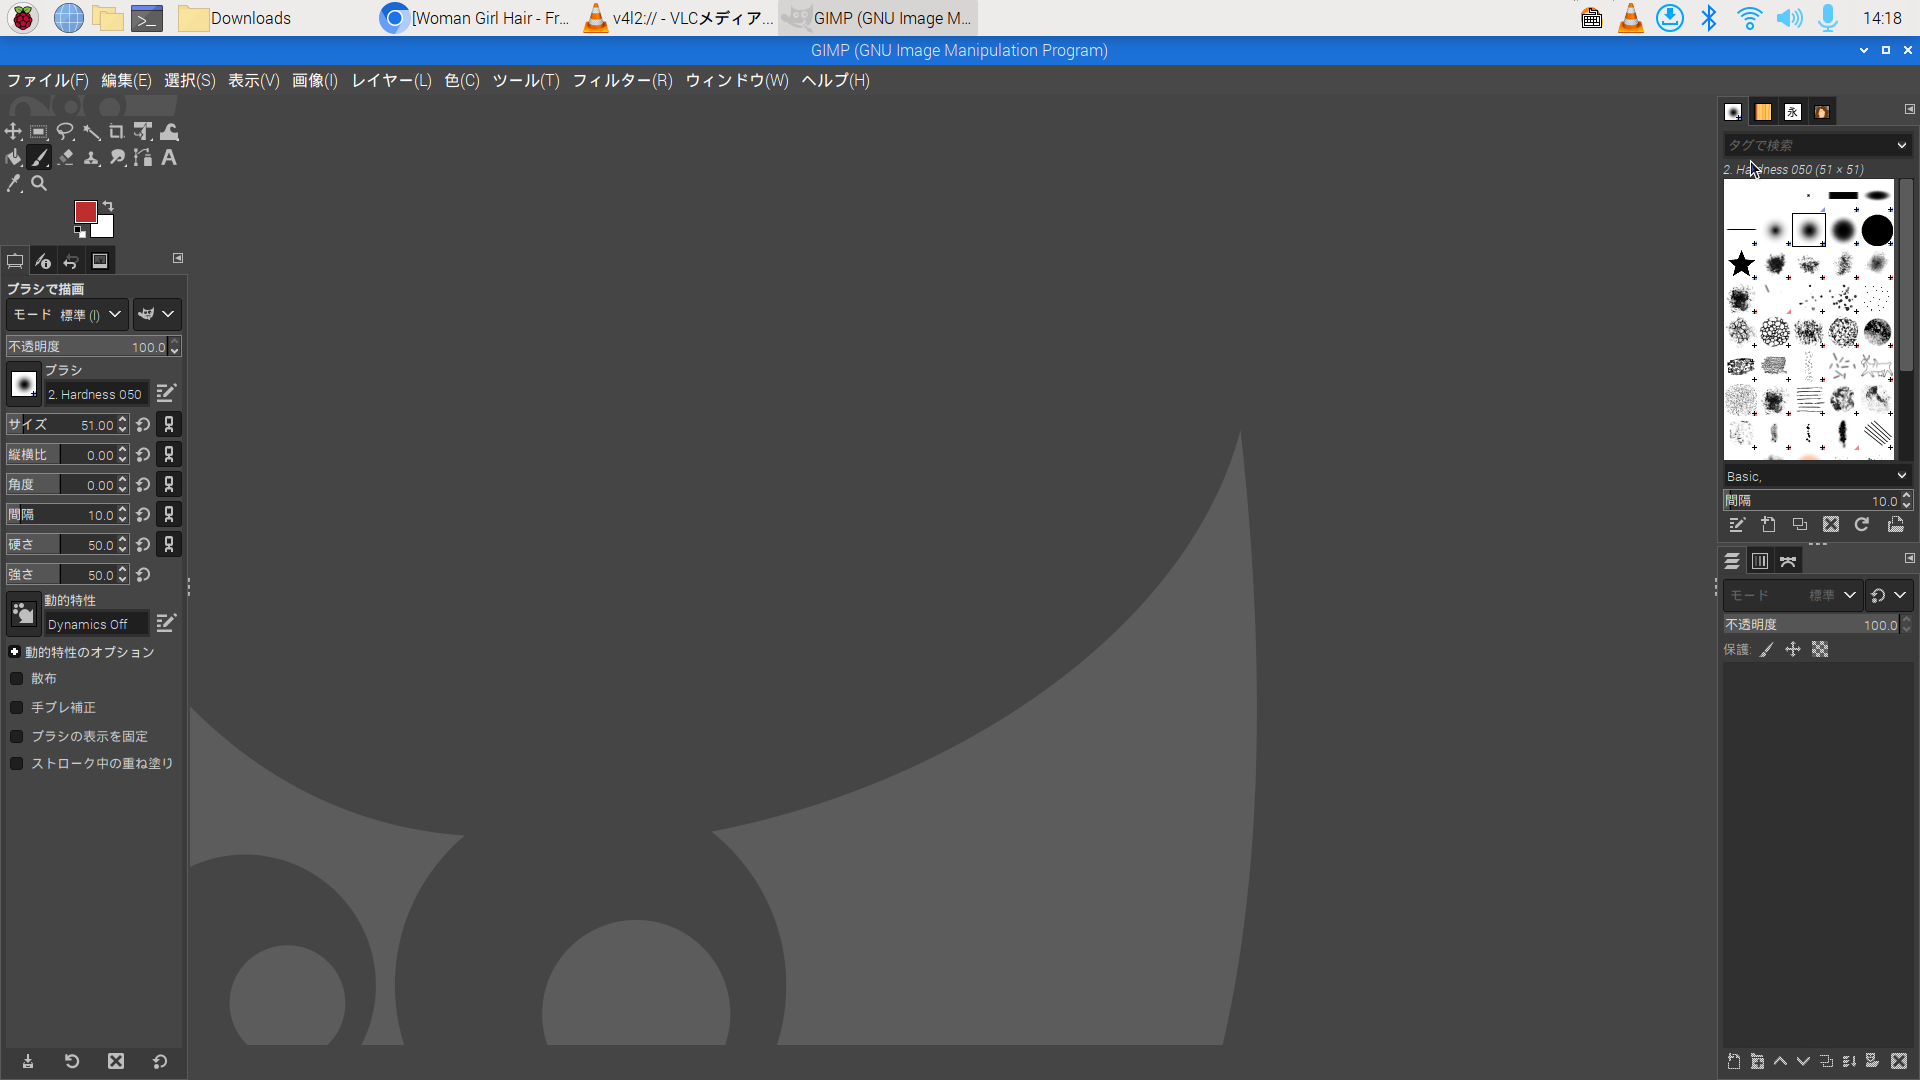
\includegraphics[width=\linewidth]{text01-img/textbook-img1032.png}\\
      17 \ruby{画像}{がぞう}が消え、何もないウィンドウになります。右上の×ボタンをクリックして、\ruby{画像}{がぞう}\ruby{編集}{へんしゅう}ツールを閉じましょう
    \end{minipage}
  \end{minipage}

  \bigskip
  \begin{minipage}{0.45\linewidth}
    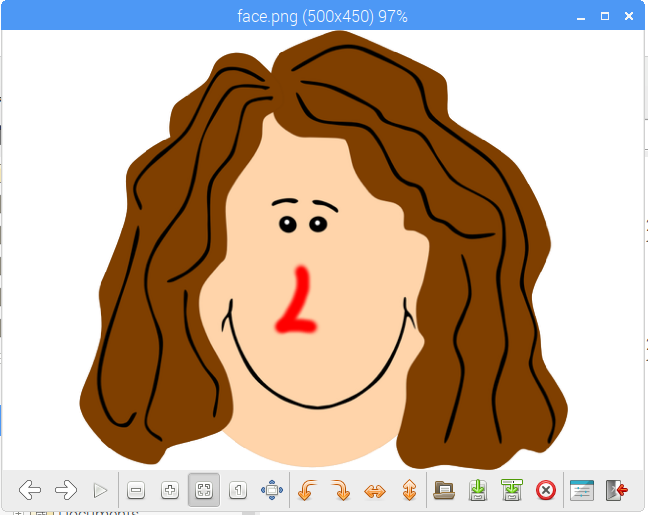
\includegraphics[width=0.9\linewidth]{text01-img/textbook-img139.png}\\
    18 \ruby{画像}{がぞう}ファイルを開いて\ruby{確認}{かくにん}してみよう
  \end{minipage}
  \vskip.5\baselineskip
  \noindent \textbf{問題 1-16}\\
  ”GIMP”を使って、自分の顔写真をさらに\ruby{編集}{へんしゅう}、加工してみよう

  \centering
  \begin{minipage}{0.5\textwidth}
    {\upshape
      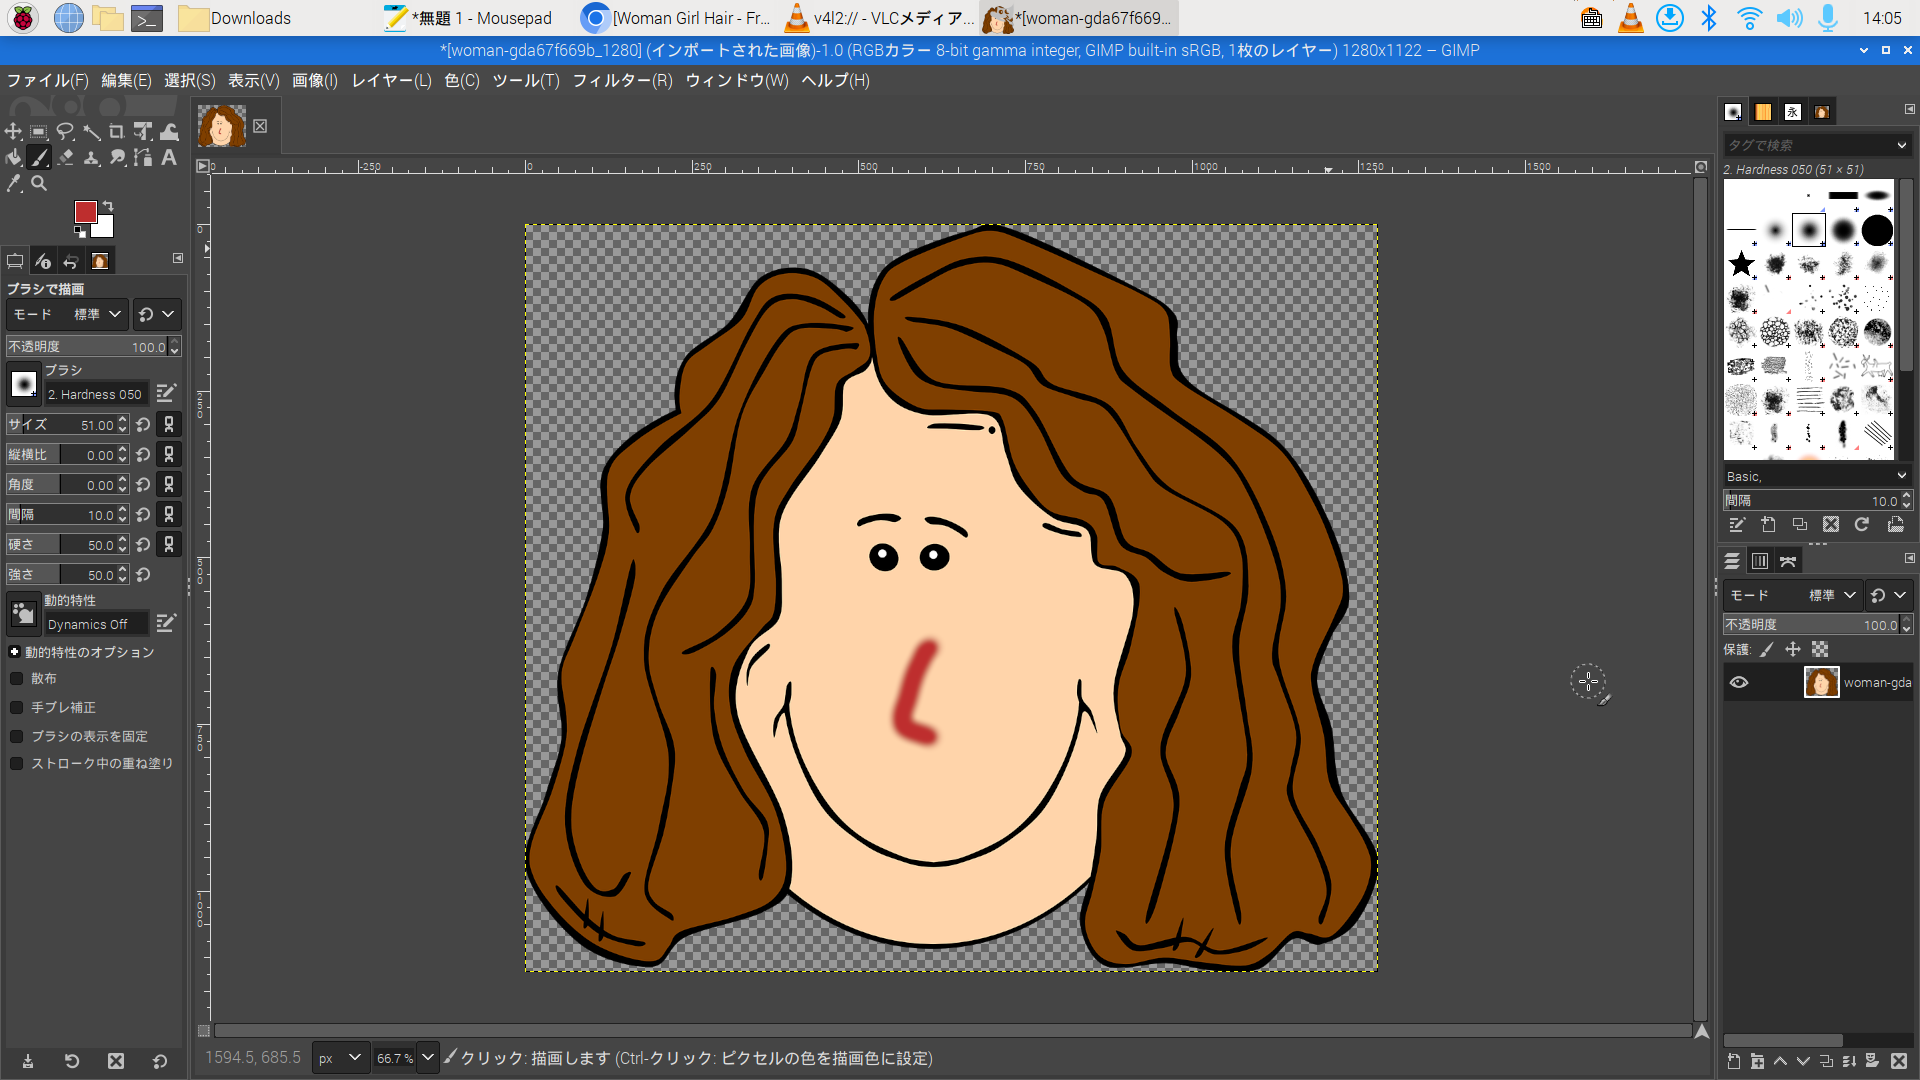
\includegraphics[width=\linewidth]{text01-img/textbook-img131.png}
      \caption{GIMP\ruby{画像}{がぞう}\ruby{編集}{へんしゅう}}
    }
  \end{minipage}
\end{figure}


\clearpage

